\label{chap:arch}

The implementation of the algorithm presented in this article is a system of two individual 
specialized algorithms which work together in order to achieve a clear and easy to follow drawing for a given graph.
 These components are: the placing algorithm, which is responsible for putting each node in a location
which facilitates the routing process, and the routing algorithm, which traces the
connections between the nodes. 

The output of these algorithms is displayed using a Java technology library called Draw2D \cite{wurthinger2006visualization}.
This library provides an API which allows the programmer to draw various shapes and forms or
embed external components such as images into a canvas. The advantages of using such a 
library instead of directly drawing on the canvas with native functions is that the entire
drawing process is transparent to the programmer. The library only requires essential 
information regarding what the shapes will be and where they are located. This allows for 
more effort to be directed towards the implementation of the core components of the system
rather than towards a secondary part such as this.

The graphs are read by the system from input files. These files contain natural-like
representations of the graph. In essence, they are lists which specify the characteristics
of each node, such as ports (which are inputs, which are outputs, which shall not be 
connected etc.) and which are the nodes that will be connected with it.

After being read, this data is passed to the placing algorithm. Here, it shall be processed 
according to the specified heuristics and shall obtain the optimal locations for all the
nodes. This solution, however, is not the global optimal solution for the given problem. At 
this point, the system may be asked to re-evaluate the result and obtain new locations. Given
that each solution is merely an approximation, the new set of positions may be completely
different for certain elements.

Finally, after having places each node, the system passes this data to the routing algorithm.
Here, the connections will be determined in regard to the specified restrictions. The result of 
this step is the information about each node and connection which is needed by the graphical
library functions to draw the graph.

\begin{figure}[ht] \centering
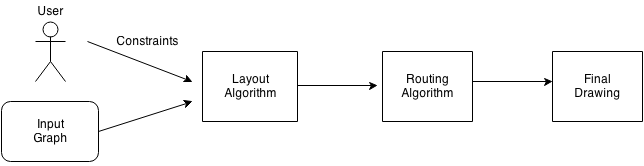
\includegraphics[width=0.5\textwidth]{src/systemWorkflow.png}
\caption{Routing algorithm workflow} \end{figure}
